\documentclass{beamer}

\newcommand\tab[1][1cm]{\hspace*{#1}}
\usepackage[spanish]{babel}
\usepackage[utf8]{inputenc}
\usepackage{bussproofs}
\usepackage{url}
\usepackage[document]{ragged2e}
\usepackage{tikz}
\usetikzlibrary{shapes,arrows,spy,positioning,snakes}
\usepackage{verbatim} % comentarios
\usepackage{tabulary} % tablas

\DeclareOptionBeamer{compress}{\beamer@compresstrue}
\ProcessOptionsBeamer

\mode<presentation>

\useoutertheme[footline=authortitle]{miniframes}
\useoutertheme{infolines}
\useinnertheme{circles}
\usecolortheme{whale}
\usecolortheme{orchid}

\definecolor{beamer@blendedblue}{rgb}{0.137,0.466,0.741}

\setbeamercolor{structure}{fg=beamer@blendedblue}
\setbeamercolor{titlelike}{parent=structure}
\setbeamercolor{frametitle}{fg=black}
\setbeamercolor{title}{fg=black}
\setbeamercolor{item}{fg=black}

\setbeamertemplate{bibliography item}[text]

\mode
<all>

\title[]{Commercial paper}
\subtitle{Fundamentos de blockchains}
\author{René Dávila - Jorge Solano}
%\institute{IIMAS}
\date{ }

\AtBeginSection[] { 
	\begin{frame} 
		\frametitle{Índice}
		\tableofcontents[currentsection]
	\end{frame}
}
\AtBeginSubsection[] { 
	\begin{frame}
		\frametitle{Índice}
		\tableofcontents[currentsection, currentsubsection]
	\end{frame}
}

\setbeamertemplate{navigation symbols}{}

\begin{document}
	\EnableBpAbbreviations
	
	\begin{frame}
		\begin{center}
			
\includegraphics [width =0.2 \textwidth ]{iimas}
		\end{center}
		\titlepage 
	\end{frame}

	\section{Commercial paper}
	
	\begin{frame}
		Diagrama de las organizaciones:
		\begin{figure}[h]
			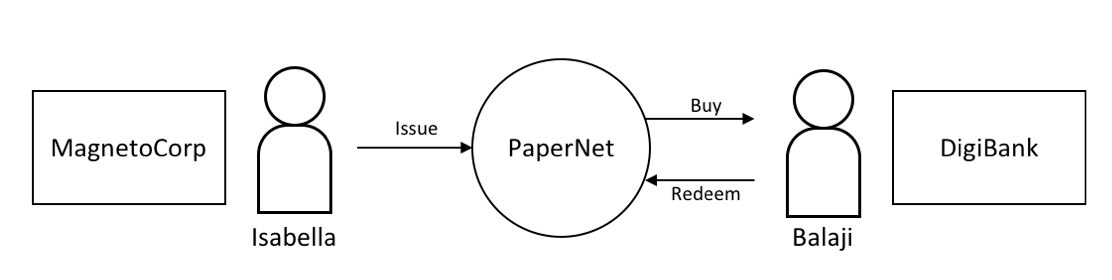
\includegraphics[scale=.5]{papernet_01}
			\centering
		\end{figure}
		Las organizaciones MagnetoCorp y DigiBank intercambian papeles comerciales en la red PaperNet.
	\end{frame}
	
	\subsection{PaperNet}

	\begin{frame}
		\frametitle{Peers y canal de comunicación}
		En cd fabric-samples/test-network:\\
		\begin{center}
			\begin{tabulary}{\linewidth}{L}
				\hline
				(PaperNet admin)\$ ./network.sh up \\
				\hline 
				(PaperNet admin)\$ ./network.sh createChannel \\
				\hline
			\end{tabulary} 
		\end{center}
	\end{frame}
	
	\begin{frame}
		\frametitle{Red docker net\_test}
		En cd fabric-samples/commercial-paper\\
		\begin{center}
			\begin{tabulary}{\linewidth}{L}
				\hline
				(PaperNet admin)\$ ./network-starter.sh \\
				\hline 
				(PaperNet admin)\$ docker ps \\
				\hline
				(PaperNet admin)\$ docker network inspect net\_test \\
				\hline
			\end{tabulary} 
		\end{center}
		peer0.org1.example.com $\rightarrow$ DigiBank\\
		peer0.org2.example.com $\rightarrow$ MagnetoCorp
	\end{frame}

	\begin{frame}
		\frametitle{Monitorear la red como MagnetoCorp}
		En cd commercial-paper/organization/magnetocorp\\
		\begin{center}
			\begin{tabulary}{\linewidth}{L}
				\hline
				(MagnetoCorp admin)\$ ./monitordocker.sh net\_test [port\_number] \\
				\hline
			\end{tabulary} 
		\end{center}
	\end{frame}
	
	\subsection{Chaincode}
	
	\begin{frame}
		\frametitle{Código del smart contract}
		En cd commercial-paper/organization/magnetocorp\\
		\begin{center}
			\begin{tabulary}{\linewidth}{L}
				\hline
				(MagnetoCorp dev)\$ code contract \\
				\hline
			\end{tabulary} 
		\end{center}
	\end{frame}

	\begin{frame}
		\frametitle{Ciclo de vida en Fabric}
		\begin{figure}[h]
			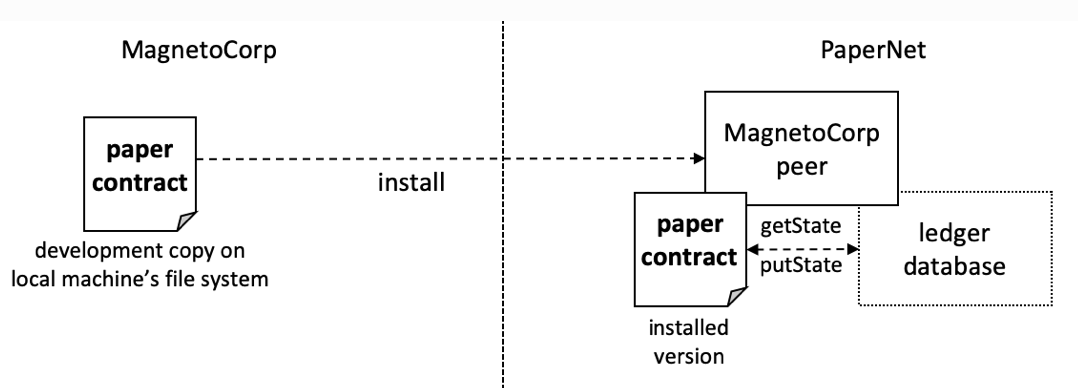
\includegraphics[scale=.4]{papernet_02}
			\centering
		\end{figure}
		\begin{itemize}
			\item El desarrollador empaqueta el chaincode ([1...n] smart contract)
			\item El administrador instalar el chaincode en cada organización.
			\item El administrador de cada organización debe aprobar el chaincode.
			\item El administrador publica en el chaincode en el ledger del canal asociado.
		\end{itemize}
		{\tiny \url{https://hyperledger-fabric.readthedocs.io/en/release-2.0/chaincode\_lifecycle.html\#chaincode-lifecycle} }
	\end{frame}
	
	\begin{frame}
		\frametitle{Instalación y aprobación en MagnetoCorp}
		En cd commercial-paper/organization/magnetocorp\\
		\begin{center}
			\begin{tabulary}{\linewidth}{L}
				\hline
				(MagnetoCorp dev)\$ code contract \\
				\hline
			\end{tabulary} 
		\end{center}
	\end{frame}
	
	\section{Referencias}
	
	\begin{frame} [allowframebreaks]
		\frametitle{Referencias}
		\begin{itemize}
			\item \url{https://hyperledger-fabric.readthedocs.io/en/release-2.0/tutorial/commercial\_paper.html\#prerequisites}
		\end{itemize}
	\end{frame}
\end{document}